Machine learning is currently a hot topic for many reasons. The most important is that it can recognize unknown patterns and make decisions based on data-driven predictive models without being explicitly programmed to do so.

There are obvious questions that need to be answered to implement machine learning systems properly. Having several algorithms to choose from, the answer to these questions varies depending on different situations as no single algorithm works for all of them. There are many factors at work, such as the size and structure of the available data, the purpose of using machine learning in that particular scenario, and the available computational power. This section provides a better understanding of the multiple paradigms, tasks, and the most common machine learning algorithms currently available.

\subsection{Learning Process Overview}

Machine learning algorithms rely on historical data (i.e., a data set) typically represented as a table, where each row represents an instance or data point. Each column represents the features of that instance and its corresponding values. 

The data set is usually split into at least two different subsets, a training data set, in which a predictive model is built from, and a test data set to determine the model's predictive accuracy. Usually, an optional third validation set may be created as well.

As mentioned earlier, machine learning algorithms use statistics and mathematical optimization to automatically find unknown data patterns and predict some target output or response. The optimization process generally involves finding the minimum or maximum value of a function, often referred to as a loss or cost function.

\subsection{Types of Learning Algorithms}

Different machine learning algorithms differ in their approach, the type of data used as input and output, and the type of task or problem they are intended to solve. This subsection discusses the different types of algorithms available.

\subsubsection{Supervised Learning}

In supervised learning, the input data has a known label or result. The goal is to predict a target variable of the unseen data given a set of variables or features. The algorithms build a predictive model on labeled historical data and learn relationships between the input and label variables. Table \ref{tab:supervised_learning} shows a typical simple example of a supervised learning problem, where the target variable to be predicted is the class of the iris plant.

\begin{table}[H]
\begin{tabular*}{\textwidth}{p{0.17\textwidth} p{0.17\textwidth} p{0.17\textwidth} p{0.17\textwidth} p{0.20\textwidth}}
\hline
\multicolumn{4}{c}{\textbf{Features}}                                                                                                               & \textbf{Target Variable}  \\ \hline
\textit{\textbf{Sepal Length}} & \textit{\textbf{Sepal Width}} & \textit{\textbf{Petal Length}} & \textit{\textbf{Petal Width}} & \textit{\textbf{Species}} \\ \hline
5.1                                 & 3.5                                & 1.4                                 & 0.2                                & setosa                    \\
4.9                                 & 3.0                                & 1.4                                 & 0.2                                & setosa                    \\
4.7                                 & 3.2                                & 1.3                                 & 0.2                                & setosa                    \\
4.6                                 & 3.1                                & 1.5                                 & 0.2                                & setosa                    \\
5.0                                 & 3.6                                & 1.4                                 & 0.2                                & setosa                    \\ \hline
\end{tabular*}
\caption{Example of supervised learning naming conventions}
\label{tab:supervised_learning}
\end{table}

A predictive model's quality is measured using an independent test set to evaluate whether the discovered relationships are helpful in unseen scenarios. By feeding the model with input variables of the test data, it is possible to compare its predicted label with the data's actual label. The evaluation process typically involves a proportional split between train and test data. A more significant proportion of test data ensures a better performance validation. In contrast, insufficient training data means that the model has fewer data to learn from.

\subsubsection{Unsupervised Learning}

Unsupervised learning involves learning from data with no label or response variable and is more about finding patterns than prediction. It is referred to as unsupervised since it lacks a response variable that can supervise the analysis. Considering that no labels are available for input data, a model is built by deducting hidden input data patterns.

\subsubsection{Reinforcement Learning}

The reinforcement learning approach is illustrated in Figure \ref{fig:reinforcement_learning}. The algorithm interacts with an environment and learns to optimize its behavior over a continuous feedback system of rewards and punishments to maximize the numerical value of reward over a given amount of time.

\begin{figure}[H]
\centering
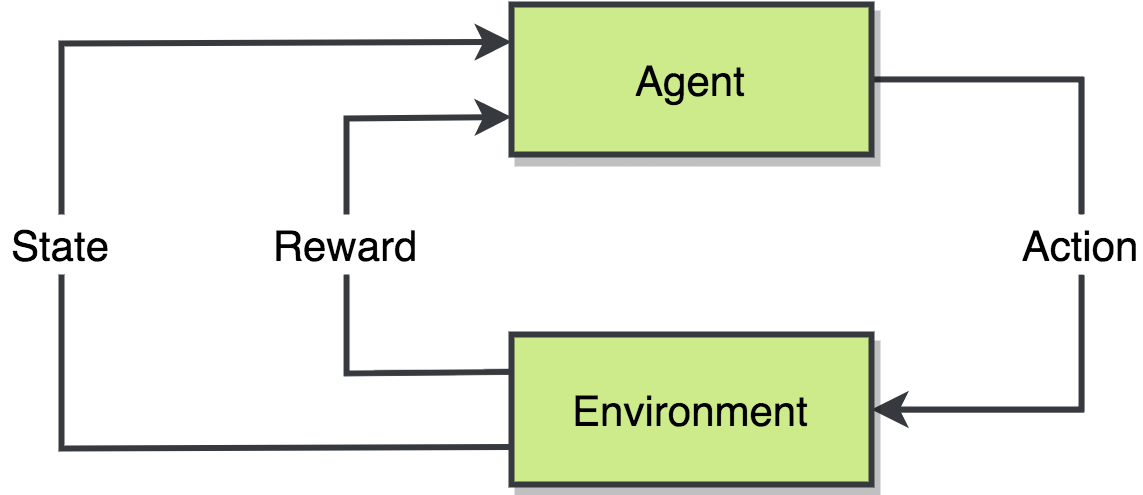
\includegraphics[width=0.6\textwidth]{img/state_of_the_art/reinforcement_learning.png}
\caption{Reinforcement learning}
\label{fig:reinforcement_learning}
\end{figure}

In contrast to supervised learning, the agent observes the current state and decides what to do, predicting the expecting future, so the agent is bound to learn from its experience. Reinforcement learning focuses on online planning and requires a balance between exploration (of the unknown) and exploitation (of existing knowledge).

\subsection{Tasks}
\label{sec:machine_learning_tasks}

A machine learning task refers to the type of prediction or inference being made based on the problem or question being asked and the available data. This subsection describes the different machine learning tasks and some of their conventional use cases.

\subsubsection{Classification}

Classification is a supervised machine learning task in which one or more classes are assigned to each instance based on a set of values for the input variables. It has different types depending on the number of output classes available: binary classification when there are two classes and multi-class classification when there are three or more classes. It is important to note that it differs from multi-label classification, where an instance can be assigned to multiple labels.

\subsubsection{Regression}

Target variables can be either numerical or categorical. While classification problems are associated with categorical labels, regression tasks refer to problems with a numerical target variable. Regression algorithms model how the variation in the values of features translates into a numerical label.

\bigbreak

\noindent Even though classification and regression are the most popular tasks, there are other types of tasks worth mentioning:

\begin{itemize}
    \item \textbf{Clustering} where the main goal is to group instances of data into clusters that contain similar characteristics by identifying relationships in a data set that one can not merely derive by browsing or simple observation;
    \item \textbf{Anomaly Detection} that identifies rare events or observations that differ significantly from the majority of the data;
    \item \textbf{Recommendation Systems} that can produce a list of recommended products or services to a given user. These systems can use a single input or multiple inputs within and across platforms, such as items, users, and transactions.
\end{itemize}

\subsection{Algorithms}
\label{sec:machine_learning_algorithms}
There are many algorithms proposed in the literature, each with its advantages and limitations depending on the task at hand and the data available. Commonly used machine learning algorithms include:

\subsubsection{Linear \& Logistic Regression}

Regression algorithms infer the relationship between output labels and the corresponding input data features. The main difference between linear and logistic regression relies on the type of dependent variable. In linear regression, it is continuous, while in logistic regression, it is discrete.

\subsubsection{Decision Trees}

Decision trees are used for both regression and classification problems based on the data's actual attributes. Each node represents a feature of a given instance, and each branch represents a decision. The leaves represent an outcome, which can be either categorical or numerical.

\subsubsection{Association Rules}

Association rule learning algorithms are a form of rule-based machine learning method to discover associations between data variables. Each rule is formed of an antecedent and a consequent, enabling the discovery of frequent patterns or association structures within a data set.

\subsubsection{Support Vector Machines}

Support Vector Machine can be used for both classification and regression problems and divides the data samples of two classes by determining a hyper-plane in input space that maximizes the separation between them and classifies new cases to one of the two groups.

\subsubsection{Genetic Algorithms}

Genetic Algorithms view learning in terms of competition among a population of evolving, alternative concepts. A genetic algorithm maintains a population of candidate problem solutions. According to their performance, only the fittest of these solutions survive and exchange information with other candidates to form new solutions.

\subsubsection{Artificial Neural Networks}

Artificial Neural Networks, inspired by biological neural networks, comprise basic processing units called neurons, connections, and weights. During the learning process, the weights of the connections are updated over time using a backpropagation algorithm to model the dependencies between input features and target variables.

Deep learning refers to a large and deep artificial neural network with many more layers and many more nodes in each layer, resulting in many more parameters to tune.
The higher amount of available data and computational power are the reason for its sudden popularity over the years.

\paragraph{Convolutional Neural Networks}

A convolutional neural network (\gls{cnn}) is a particular type of neural network that takes an image as input. It can differentiate one image from the other by assigning importance through learnable weights and biases to various traits or objects in the image. As illustrated in Figure \ref{fig:convolutional_neural_networks}, it has convolutional layers that intend to capture the high-level features from the input image, and pooling layers, responsible for reducing images into an acceptable size that is easier to process without losing the convolved feature, which is a critical step for getting the right prediction.

\begin{figure}[H]
\centering
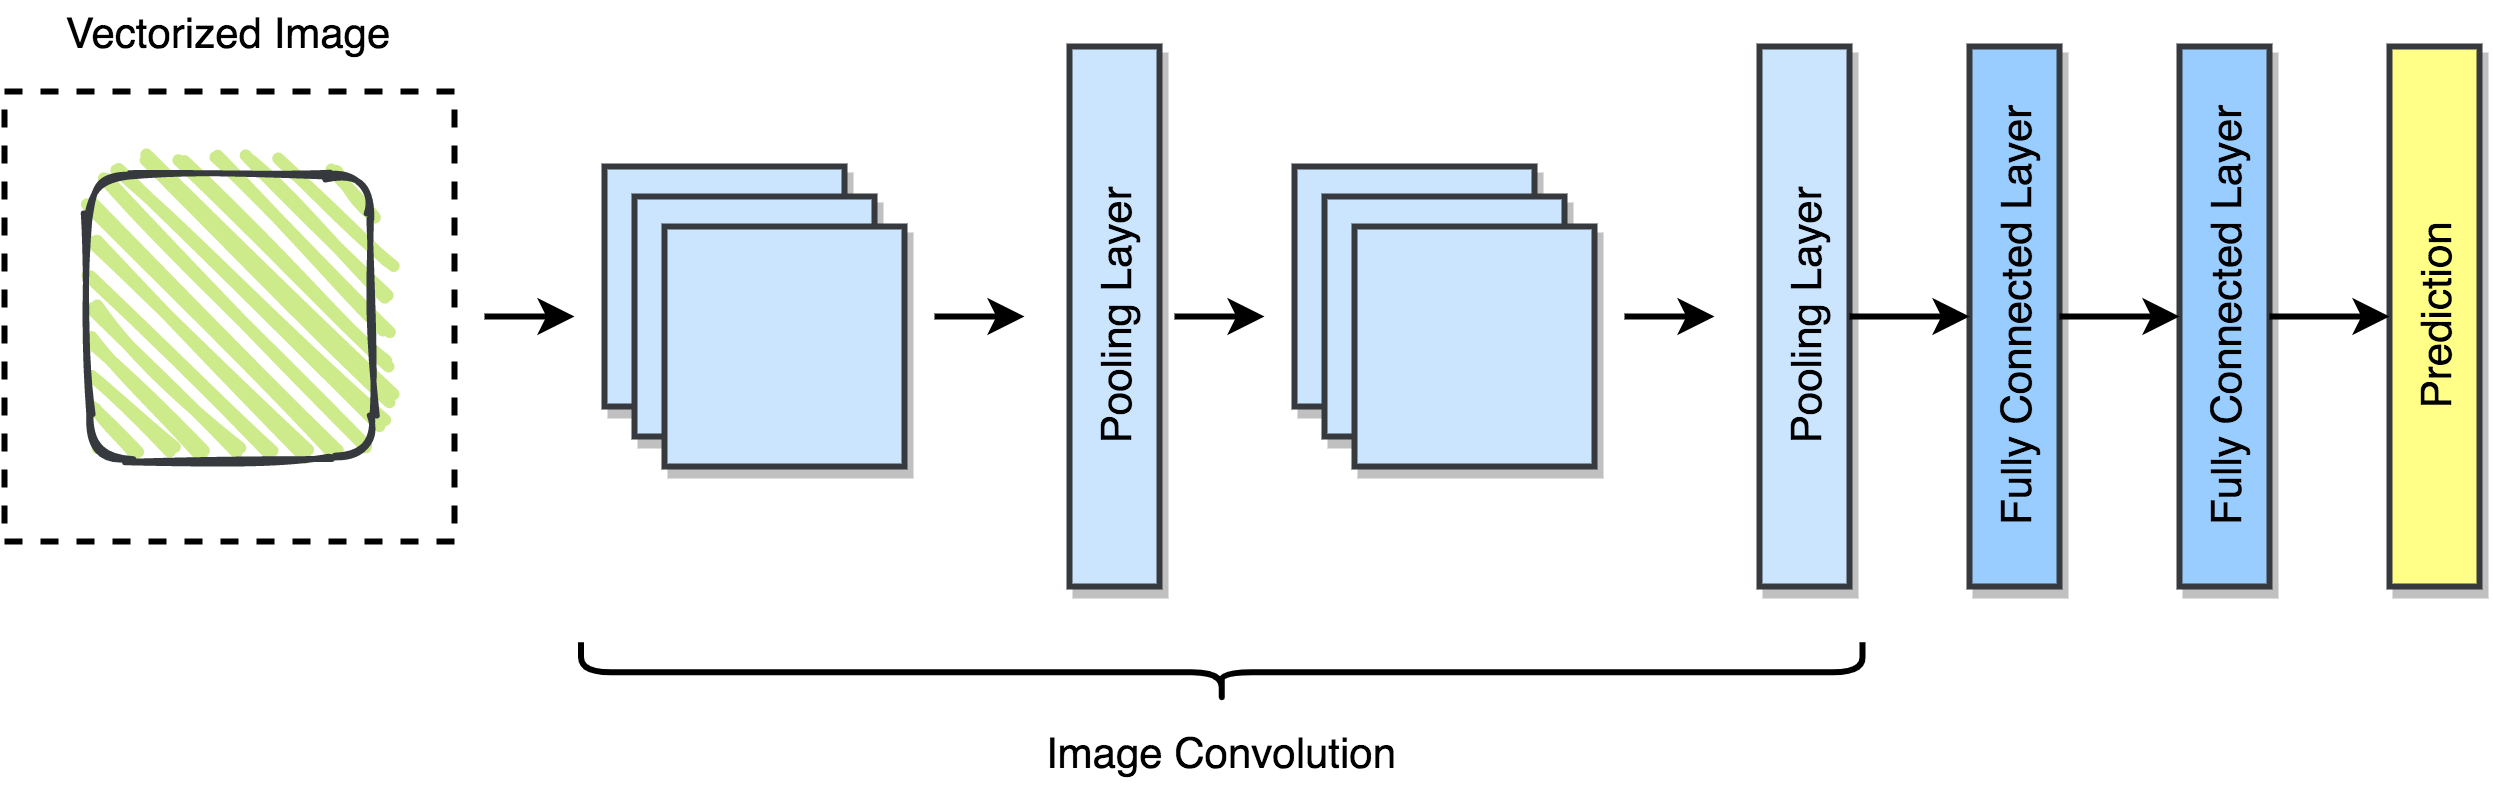
\includegraphics[width=\textwidth]{img/state_of_the_art/convolutional_neural_network.png}
\caption{Convolutional neural networks}
\label{fig:convolutional_neural_networks}
\end{figure}

The actual learning process is done by feeding the flattened output of the high-level features (i.e., the convolutional layer's output) to a feed-forward neural network and applying the backpropagation algorithm to every training iteration. Thus, over a series of epochs, the model can distinguish between dominating and certain low-level features in images.